\chapter{The LHC and the CMS Detector}
\label{chap:LHC}
\section{Large Hadron Collider}
The Large Hadron Collider (LHC)\cite{lhc} is a circular synchrotron with a
circumference of \unit{27}{\kilo\meter}.  It has been constructed in the
existing tunnel \unit{40-170}{\meter} beneath the border of France and
Switzerland that was previously home to the LEP collider \cite{myers1990design}.

When operating at its design energy and luminosity it will collide beams of
protons at a centre of mass energy of \unit{14}{\TeV} and a luminosity of
\unit{$ 10^{34} $}{\rpsquare\cm\reciprocal\second}.  It is also designed to
collide two \unit{5.5}{\TeV} beams of lead ions, and other species\cite{lhc}.
\TableRef{tab:lhcparam} summarises the machine parameters relevant to the {CMS}
detector.

\begin{table}[htbp]
\begin{center}
\begin{tabular}{ l l l }
\toprule
Parameter & p-p & Pb-Pb \\
\midrule
Energy per nucleon ($\TeV$)& 7 & 2.36 \\
Dipole field at \unit{7}{\TeV} ($\tesla$)& 8.33 & 8.33\\
Design luminosity ($\lumiunits$)& $10^{34}$ & $10^{27}$ \\
Bunch separation ($\ns$)& 25 & 100\\
No. of bunches & 2808 & 592 \\
No. particles per bunch& $1.15\times10^{11}$ & $1.15\times10^{11}$\\
\midrule
$\beta$-value at IP ($\metre$)& 0.55 & 0.5 \\
RMS beam radius at IP ($\micron$)& 16.7 & 15.9 \\
Luminosity lifetime (hr)& 15 & 6 \\
Average number of collisions/crossing & 20 & - \\
\bottomrule
\end{tabular}
\caption[The machine parameters relevant for the LHC detectors.]
{The machine parameters relevant for the LHC detectors. From \cite{chatrchyan2008cms}.}
\label{tab:lhcparam}
\end{center}
\end{table}

The main motivation for the LHC is to determine the mechanism that is
responsible for electroweak symmetry breaking, of which the most favoured is the
Higgs mechanism.  The LHC is also designed to test the Standard Model at the
$\TeV$ scale at high precision and to search for new particles predicted by
theories beyond the Standard Model such as supersymmetric theories and theories
involving extra dimensions.  \FigureRef{fig:LHCxsec} shows various cross
sections for several physics processes as a function of the centre of mass
energy. The cross section for many physics processes of interest, such as the
Higgs cross section, $\sigma_{Higgs}$, are many orders of magnitude lower than the
total inelastic cross section, $\sigma_{tot}$, and increase as a function of
centre of mass energy.  The large centre of mass energy and high luminosity of
the LHC is needed to be able to probe the physics processes of interest with
small cross sections.

\begin{figure}[htbp]
  \centering
  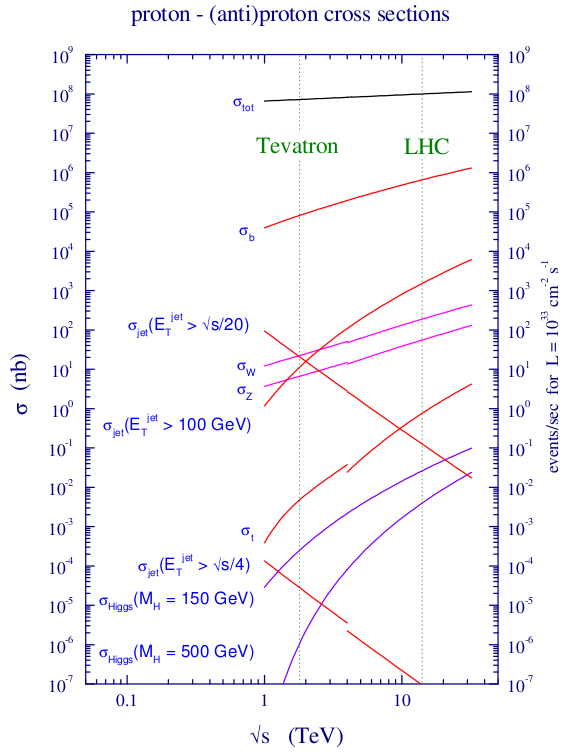
\includegraphics[width=0.85\textwidth]{xsec.png}
  \caption[The theoretical production cross sections as a function of centre of
mass energy for several Standard Model processes.] {The theoretical production
cross sections as a function of centre of mass energy for several Standard Model
processes such as the b quark production cross section, $\sigma_{b}$, and the
Higgs boson production cross sections, $\sigma_{Higgs}$.  $\sigma_{tot}$ is the
total inelastic cross section.  The cross sections that are of relevance to this
thesis analysis are the \PW and \PZ boson cross sections $\sigma_{\PW}$ and
$\sigma_{\PZ}$ respectively.  From \cite{campbell2006hard}.}

  \label{fig:LHCxsec}
\end{figure}

The LHC is part of a larger accelerator complex as shown in 
\FigureRef{fig:LHCcomplex}. Hydrogen gas is first ionised to produce a cloud of
protons, which are then accelerated by the LINAC2 linear accelerator to
\unit{50}{\MeV}.  Before being injected into the Proton Synchrotron (PS) the
protons are injected into the Proton Synchrotron Booster (PSB) and accelerated
to \unit{1.4}{\GeV}. In the PS the protons are grouped into bunches and the
energy is increased to \unit{25}{\GeV}. The bunches are then accelerated in the
Super Proton Synchrotron (SPS) to \unit{450}{\GeV} and then injected into the
LHC.

\begin{figure}[htbp]
  \centering
  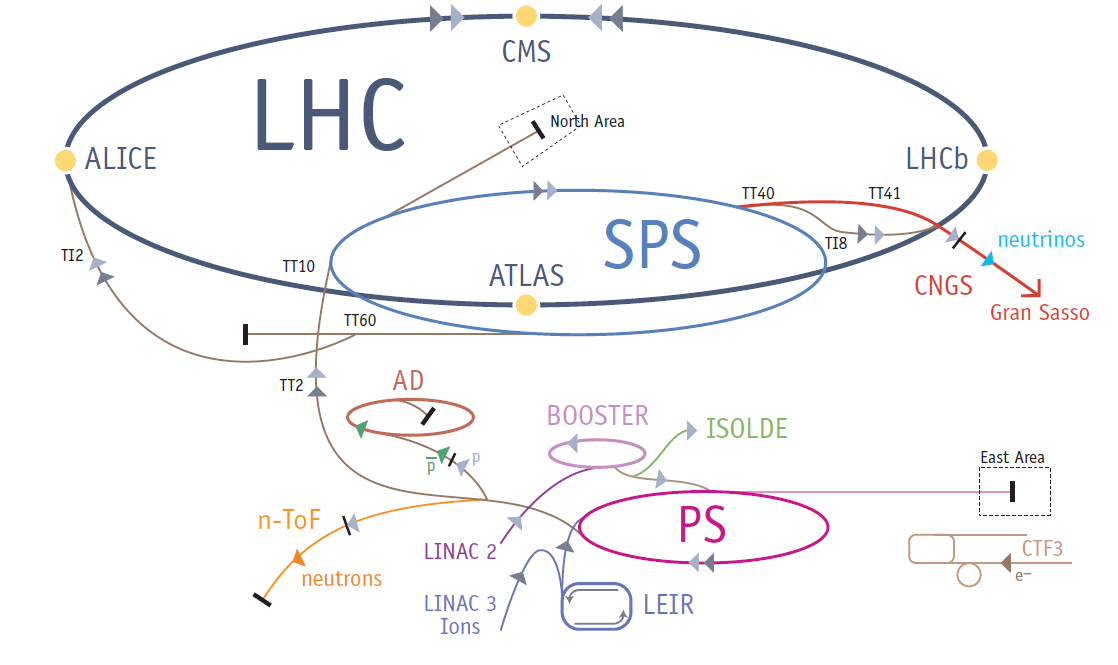
\includegraphics[width=0.96\textwidth]{accelerators.png}
  \caption{The LHC complex.}
  \label{fig:LHCcomplex}
\end{figure}

There are four main experiments studying the collisions at the
{LHC}.  
ALICE\footnote{A Large Ion Collider Experiment.} is designed to study the quark
gluon plasma that will be produced in the heavy ion collisions
\cite{aamodt2008alice}.
The LHCb\footnote{Large Hadron Collider beauty.} experiment is designed to study
B-meson decays to measure CP violation \cite{alves2008lhcb}.
ATLAS\footnote{A Toroidal LHC Apparatus.} and CMS\footnote{Compact Muon
Solenoid.} are general purpose detectors that are designed to search for a wide
range of new physics \cite{chatrchyan2008cms,aad2008atlas}.

In addition there are two smaller special-purpose detectors.
The LHCf \footnote{Large Hadron Collider forward.} is an experiment designed to
measure the neutral particles emitted in the very forward region of LHC
collisions.  The goal of the experiment is to provide data for hadron
interactions models that are used in the study of extremely high-energy
cosmic-rays \cite{adriani2008lhcf}.
The goal of the TOTEM\footnote{TOTal Elastic and diffractive cross section
Measurement.} experiment is to measure the total proton-proton
cross section and study the elastic and diffractive scattering at the LHC. The
detector is located at either side of the CMS detector \cite{anelli2008totem}.

\subsection{Operational History}
In September 2008 the {LHC} was commissioned and the first beams were
circulated.  Before the first collisions could be delivered an interconnection
between two of the dipole magnets failed. This led to
a large amount to helium rapidly evaporating which caused considerable damage to
the machine \cite{lebrun2009sector}.  Due to this incident it was decided that,
after the repairs,
the {LHC} should be run at a lower centre of mass energy of \unit{7}{\TeV} until
the quench protection system could be upgraded and the interconnections
thoroughly verified for higher currents \cite{myers2010lhc}.

The {LHC} was repaired by the end of 2009 and the first collisions at a record
energy of \unit{2.36}{\TeV} were delivered in November.  From March to November
2010 the {LHC} operated at \unit{7}{\TeV} delivering \unit{46.4}{\invpb} of
proton-proton collisions of which \unit{36.1}{\invpb} was certified for analysis
\cite{myers1990design}.  In November and December 2010 the {LHC} produced lead
ion collisions at \unit{2.36}{\TeV}.

\begin{figure}[htbp]
  \centering
  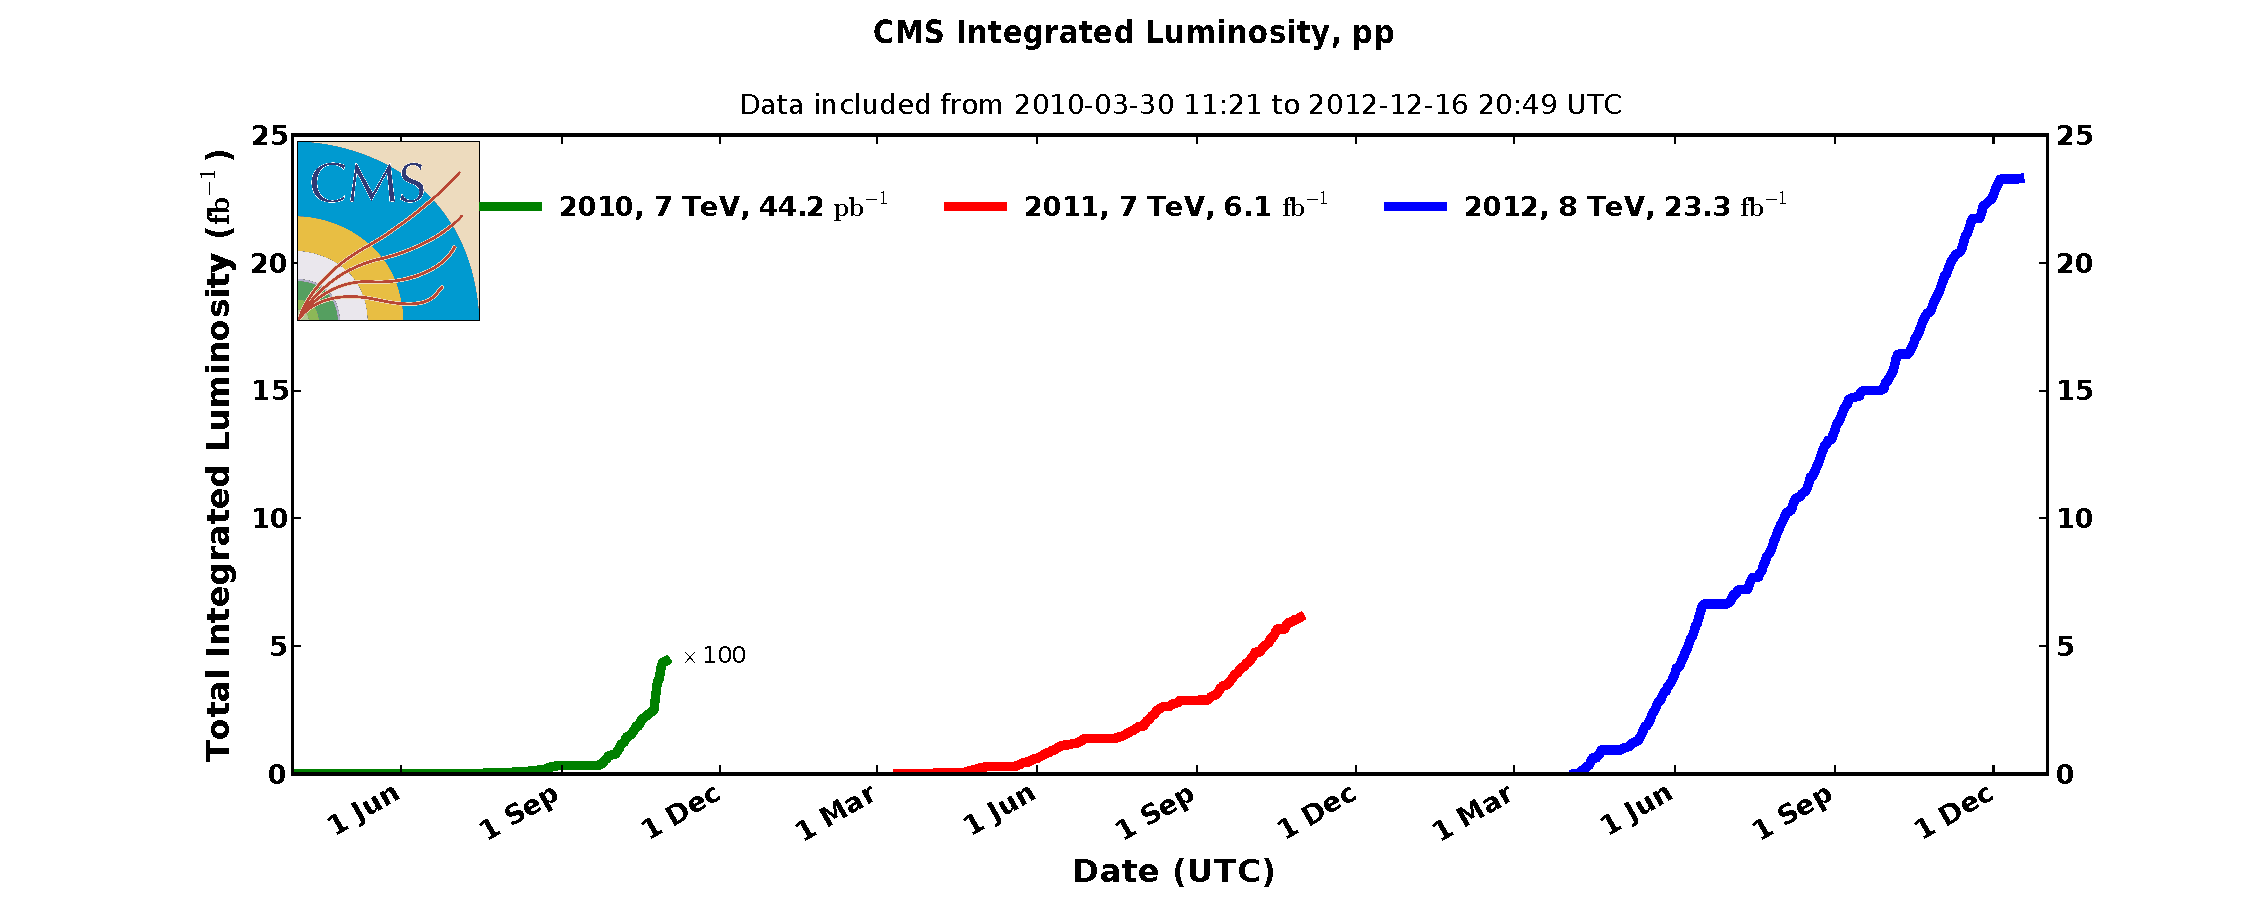
\includegraphics[width=\textwidth]{int_lumi_cumulative_pp_1}
  \caption[The luminosity delivered by LHC and recorded by CMS in 2010, 2011 and
2012.] {The luminosity delivered by LHC and recorded by CMS in 2010, 2011 and
2012. From \cite{intlumi}.}
  \label{fig:LHC2010}
\end{figure}

The target for running in 2011 was to deliver \unit{1}{\invfb} of data. This was
achieved by June. The target was increased to \unit{5}{\invfb} of data for 2011 which was achieved by October. 
In 2012 the {LHC} was operated at a centre of mass energy of \unit{8}{\TeV}
and a total of \unit{22.1}{\invfb} of data was collected by December.
The luminosity delivered by LHC and recorded in CMS in 2010, 2011 and 2012 is
shown in \FigureRef{fig:LHC2010} \cite{intlumi}.

The analysis presented in the following chapters is based on the
\unit{36.1}{\invpb} of data from  2010 and \unit{840}{\invpb} of data from the first half of 2011.

\section{CMS Detector}
{CMS}\cite{chatrchyan2008cms} is one of the two general purpose
detectors designed to study LHC collisions. The main design parameters for the
{CMS} detectors  are listed in \TableRef{tab:cmsparam}.

\begin{table}[htbp]
\begin{center}
\begin{tabular}{ l l }
\toprule
Parameter & CMS \\
\midrule
Total weight (tons)                 & $12,500$  \\
Overall diameter (m)                & $15$  \\
Overall length (m)                  & $20$  \\
Magnetic field for tracking (T)     & $4$  \\
Solid angle for energy measurements ($\Delta\phi \times \Delta\eta$)   
                                    & $2\pi \times 9.6$  \\
Solid angle for precision measurements ($\Delta\phi \times \Delta\eta$)   
                                    & $2\pi \times 5.0$  \\
Total cost (CHF)                    & $550\times 10 ^{6}$  \\
\bottomrule
\end{tabular}
\caption[Main design parameters of the CMS detector.]{Main design parameters of
the CMS detector. From \cite{froidevaux2006general}.\label{tab:cmsparam}}
\end{center}
\end{table}

The design goals of the CMS detector are:
\begin{itemize}
  \item Good muon identification and momentum resolution and the ability to
unambiguously assign charge to muons with $\PT < \unit{1}{\TeV}$
  \item Good charged particle momentum resolution and reconstruction in the
tracker.
  \item Good electromagnetic energy resolution. 
  \item Good resolution of missing transverse energy and dijet mass.
\end{itemize}

The design of CMS meets these requirements while overcoming significant
experimental challenges.  At design luminosity, approximately 1 billion
inelastic events will occur in CMS every second, whereas CMS is limited to
storing the data of only $\approx 100 $ events within that time.  The detector
must be able to reduce this rate with a trigger to accept events that are
interesting from a physics perspective and reject events otherwise.

In addition to this challenge, each event of interest will have on average 20
inelastic events superimposed on it. This results in around 1000 charged
particles produced every \unit{25}{\ns}, which require the detectors to
have a high granularity with a good time resolution to ensure a low occupancy.
The large flux of particles will also produce high radiation levels which 
required radiation hard detectors and electronics.

\begin{figure}[htbp]
  \centering
  \includegraphics[width=0.98\textwidth]{cms_120918_02}
  \caption[Diagram of the CMS detector.] {Diagram of the CMS detector. From
\cite{SketchUpCMSGallery}.}
  \label{fig:CMSnc}
\end{figure}

An overview of the detector is shown in \FigureRef{fig:CMSnc}.  Starting at the
interaction point in the centre of the detector and moving radially outwards,
CMS comprises the pixel tracker, the silicon microstrip tracker, the
lead-tungstate electromagnetic calorimeter, the sampling brass-plate hadronic
calorimter, a \unit{4}{\tesla} superconducting solenoid magnet, an outer
hadronic calorimeter and four muon chambers.


\subsection{Magnet}
A large superconducting solenoid provides the basis for the design of the CMS
detector, and is the main structural support for the detector components in the
barrel region.

The superconducting magnet in CMS produces a \unit{4}{\tesla} field in a bore of
\unit{6}{\meter} diameter and \unit{12.5}{\meter} length.  While operating at
full current the magnet stores \unit{2.6}{\giga\joule} of energy.  A large
magnetic field is needed to give CMS a large bending power and the ability to
precisely measure the momentum of high-energy charged particles.  The solenoid
bore is large enough that the tracking detectors and the calorimetry can fit
inside it\cite{chatrchyan2008cms}.

The magnetic flux is returned through a \unit{1.8}{\meter} thick saturated iron
yoke which is interleaved with the muon detector.

\subsection{Tracking}
The inner tracker is designed to accurately and efficiently measure the
trajectories of charged particles produced in collisions at the centre of CMS.
The tracker is also required to be able to reconstruct secondary vertices from
the decay of long-lived particles.  At the design luminosity of the LHC it
is expected that every \unit{25}{\ns} an average of 1000 particles will traverse
the inner detector; therefore, it is required that the tracker has a high
granularity and a fast response while remaining resilient to radiation damage. 

\begin{figure}[htbp]
  \centering
  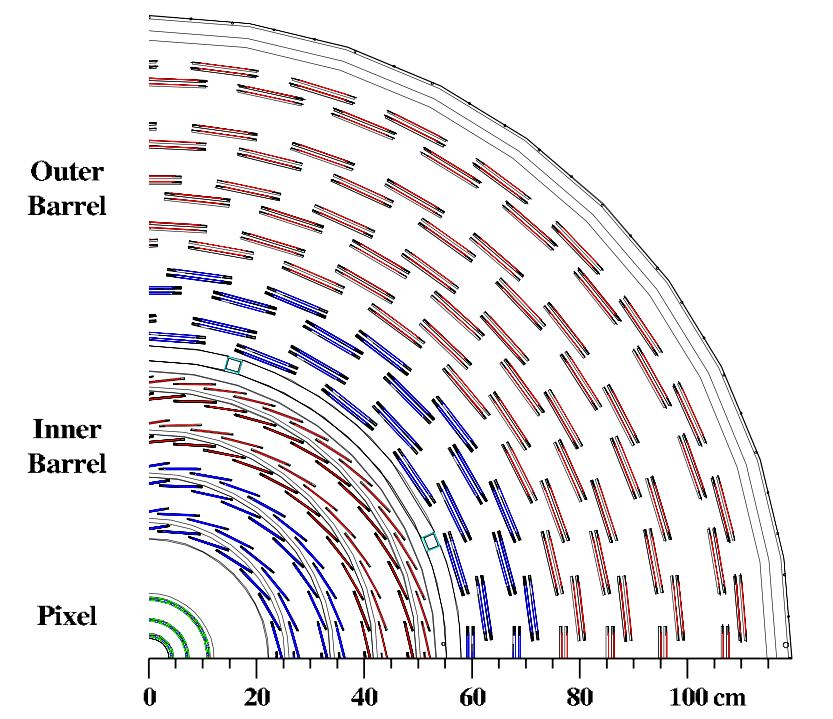
\includegraphics[width=0.7\textwidth]{tracker}
  \caption[A quadrant of the cross section of the barrel part of the {CMS}
tracker.]{A quadrant of the cross section of the barrel part of the {CMS}
tracker. From \cite{cmsgsf}.}
  \label{fig:tracker}
\end{figure}

A quadrant of the cross sections of the barrel part of the {CMS}
tracker is shown in \FigureRef{fig:tracker}.
The tracker utilises silicon pixel detectors in the innermost layers where the
particle flux is the highest.  Outside of the pixel detector, the tracking
detector comprises several layers of silicon microstrip detectors where the
particle flux is smaller.  The total active area of silicon in the CMS tracker
is over \unit{200}{\meter\squared} \cite{chatrchyan2008cms}.

\subsubsection{Pixel Tracker}
The pixel tracker consists of three layers of hybrid silicon pixel detectors in
the barrel region and two in the endcap region. 
The barrel layers are positioned at radii of 4.4, 7.3 and \unit{10.2}{\cm} and have
a length of \unit{53}{\cm}. The two layers in each endcap are located at
$|z|=34.5$ and \unit{46.5}{\cm} with an inner radius of \unit{6}{\cm} and an
outer radius of \unit{15}{\cm}.

\begin{figure}[htbp]
  \centering
  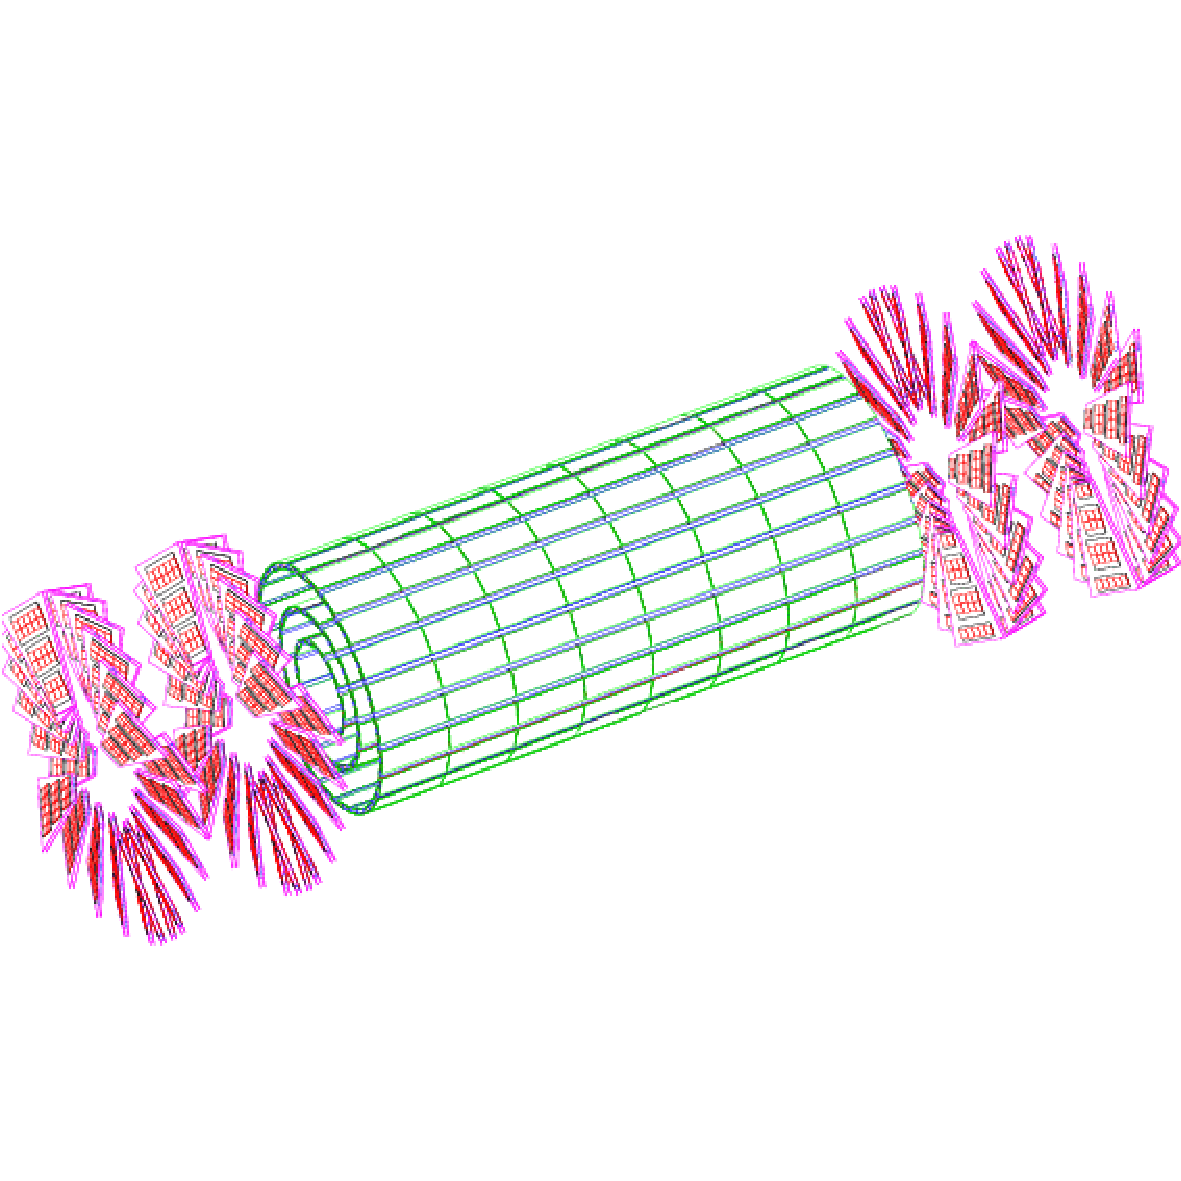
\includegraphics[width=0.98\textwidth]{pixel}
  \caption[The layout of pixel detector in the CMS tracker.]
  {The layout of pixel detector in the CMS tracker. From \cite{chatrchyan2008cms}.}
  \label{fig:pixel}
\end{figure}

A close up view of the pixel tracker is shown in \FigureRef{fig:pixel}.  
Each pixel has a surface area of \unit{$100\times150$}{\micron} which results in
an average particle occupancy of $\mathcal{O}(10^{-4})$ per pixel per crossing.

\subsubsection{Strip Tracker}
The barrel strip tracker comprises two parts, the inner (TIB) and outer (TOB)
trackers.  The TIB is made of 4 layers and covers the longitudinal region $|z|
< \unit{65}{\cm}$ and the region \unit{$20<r<55$}{\cm} in the radial direction.
The TIB utilises microstrip detectors with a cell size of
$\unit{10}{\cm}\times\unit{80}{\micron}$ with an average occupancy of
$\approx\unit{2-3}{\%}$.

The TOB is formed of 6 layers with a half-length of $|z| < \unit{110}{\cm}$. In
this region the flux is low enough to allow for the use of larger pitch
silicon microstrips with a cell size of
$\unit{25}{\cm}\times\unit{180}{\micron}$ with an average occupancy of
$\approx\unit{1}{\%}$.

The endcaps are separated into the Tracker End Cap (TEC) and the Tracker Inner
Disks (TID). The TEC is split into nine disks and covers the region
$\unit{120}{\cm} < |z| < \unit{280}{\cm}$. The TID comprises three rings
and fills the gap between the TEC and the TIB.

%\subsubsection{Performance}
%\todo[inline]{section on the performance of the tracking detectors}

\subsection{Electromagnetic Calorimeter}
The electromagnetic calorimeter (ECAL) is designed to measure the energy of
electrons and photons with a high resolution. It has a fine lateral granularity
to help with shower separation. It is a hermetic, homogeneous calorimeter
comprising 61200 individual lead tungstate ($PbWO_{4}$) scintillation crystals
in the barrel region ($|\eta|<1.479$) closed by 7324 crystals in each of the two
endcap parts ($1.479<|\eta|<3.0$) \cite{ecal1997technical}.

Lead tungstate crystals are ideally suited for this since the scintillation
decay time is similar to the LHC bunch crossing time, 
with $80\%$ of light being produced within \unit{25}{\ns}.
They also have a short radiation length ($X_0=\unit{0.89}{\cm}$) 
and Moliere radius (\unit{2.2}{\cm}) as well as being radiation hard
(up to \unit{10}{\mrad}).

A disadvantage to using lead tungstate is that the light output of the crystals
is relatively low and changes with temperature. This is overcome by using
photodetectors with an intrinsic gain and maintaining a stable temperature
(within \unit{0.1}{\degreecelsius}).

Silicon avalanche photodiodes (APDs) are used to detect the scintillation light
in the barrel and vacuum phototriodes (VPTs) are used in the endcap parts.

The barrel section of the ECAL (EB) surrounds the inner tracker. It comprises 36
identical supermodules that each cover a half length of the barrel
($0<|\eta|<1.479$) and \unit{20}{\degree} in $\phi$. Each supermodule contains 1700
crystals arranged in a $\phi - \eta$ grid with each crystal mounted in a
``semi-projective'' geometry, and aligned \unit{3}{\degree} off the nominal
interaction vertex.  The alignments in the longitudinal and transverse planes
are shown in \FigureRef{fig:crystaltilt} and \FigureRef{fig:crystallong}
respectively. The non-pointing geometry prevents particles escaping through the
gaps between the crystals \cite{ecal1997technical}.  Each crystal has a
cross section of \unit{$22 \times 22$}{\mm\squared} and a length of
\unit{230}{\mm} (\unit{25.8}{X_0}).

\begin{figure}[htbp]
  \centering
  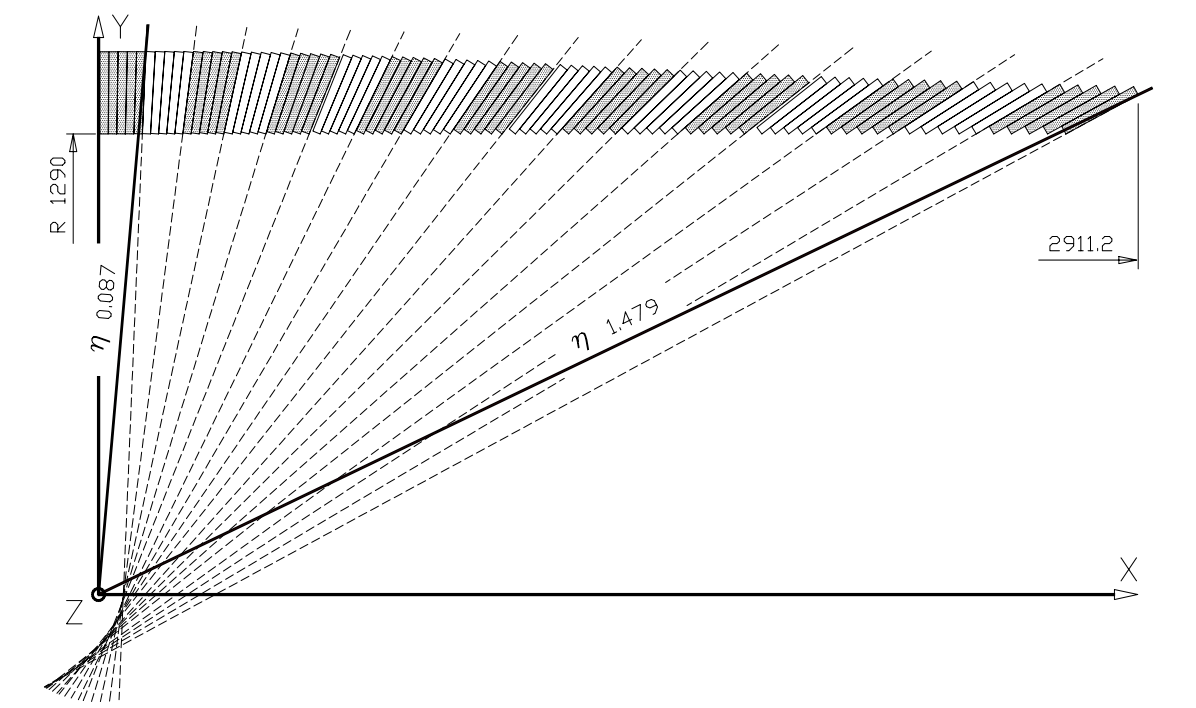
\includegraphics[width=0.8\textwidth]{crystallong}
  \caption[The crystal alignment in the longitudinal view.]{The crystal
alignment in the longitudinal view. The dotted lines show the alignment of the
edge of the crystals. A single supermodule is shown. From \cite{ecal1997technical}.}
  \label{fig:crystallong}
\end{figure}

\begin{figure}[htbp]
  \centering
  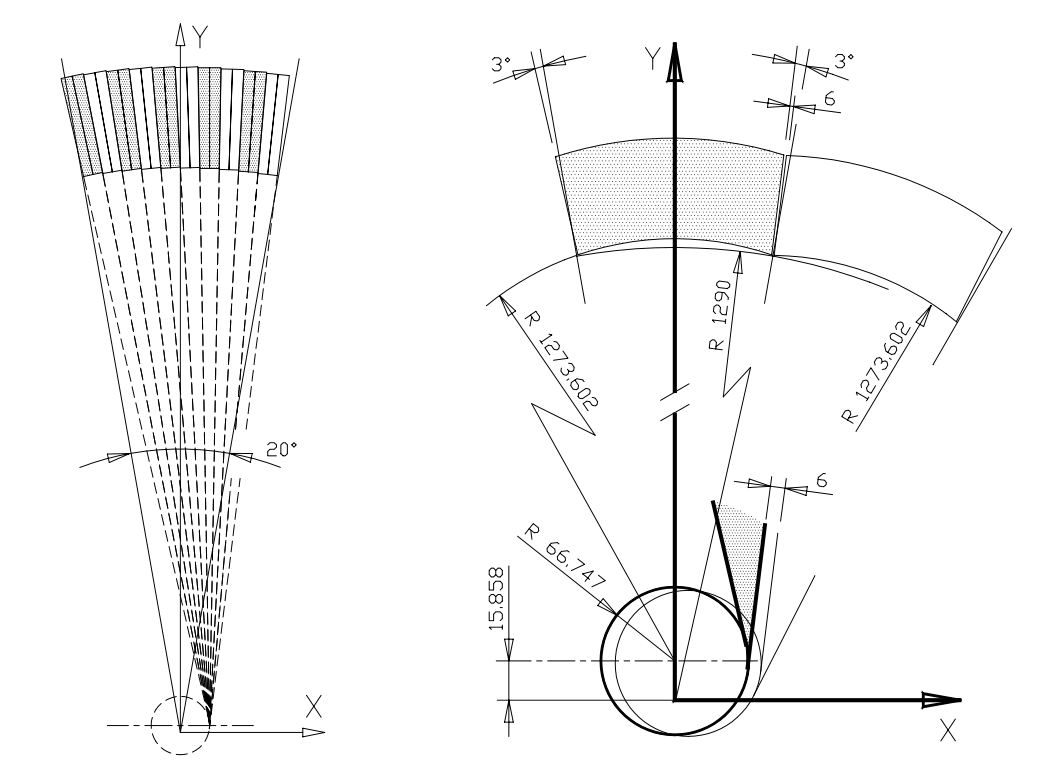
\includegraphics[width=0.8\textwidth]{crystaltilt}
  \caption[The tilt of the ECAL crystals in the transverse plane and the
alignment of the supermodules.] {The tilt of the ECAL crystals in the transverse
plane (left) and the alignment of the supermodules (right). The dotted lines
show the alignment of the crystal edges. From \cite{ecal1997technical}.}
  \label{fig:crystaltilt}
\end{figure}

The endcaps (EE) are formed of two ``Dees'', semi-circular aluminium plates
which support the ``supercrystals'', $5\times5$ arrays of crystals. The crystals are
mounted to point away from the nominal interaction vertex by a small angle in a similar way
to the barrel. 
Unlike the barrel the crystals are arranged in an $x-y$ grid.
Installed in front of the endcap ECAL is a preshower system which helps with
the rejection of \Ppizero \cite{chatrchyan2008cms}.

\subsubsection{Performance}

Using a \unit{100}{\GeV} test beam, the energy resolution of the {ECAL} was
found to be\cite{chatrchyan2008cms},
\begin{align}
\left(\frac{\sigma}{E}\right)^{2} 
&= \left(\frac{S}{\sqrt{E}}\right)^{2} + \left(\frac{N}{E}\right)^{2} + C^{2}\\
&=
\left(\frac{\unit{2}{\%}}{\sqrt{E}}\right)^{2} +
\left(\frac{\unit{124}{\MeV}}{E}\right)^{2} + 
\left(\unit{0.26}{\%}\right)^{2}  
\end{align}
where $S$ is the stochastic term, $N$ is the noise term and $C$ is the constant
term. The measured {ECAL} energy resolution is shown in \FigureRef{fig:ECAL}. The
stochastic term is due to the statistical fluctuations in the particles produced
in the electromagnetic shower. The noise term is due to electronic noise and
pile-up. The constant term is due to errors such as non-uniform signal
generation and calibration errors \cite{chatrchyan2008cms}.

\begin{figure}[htbp]
  \centering
  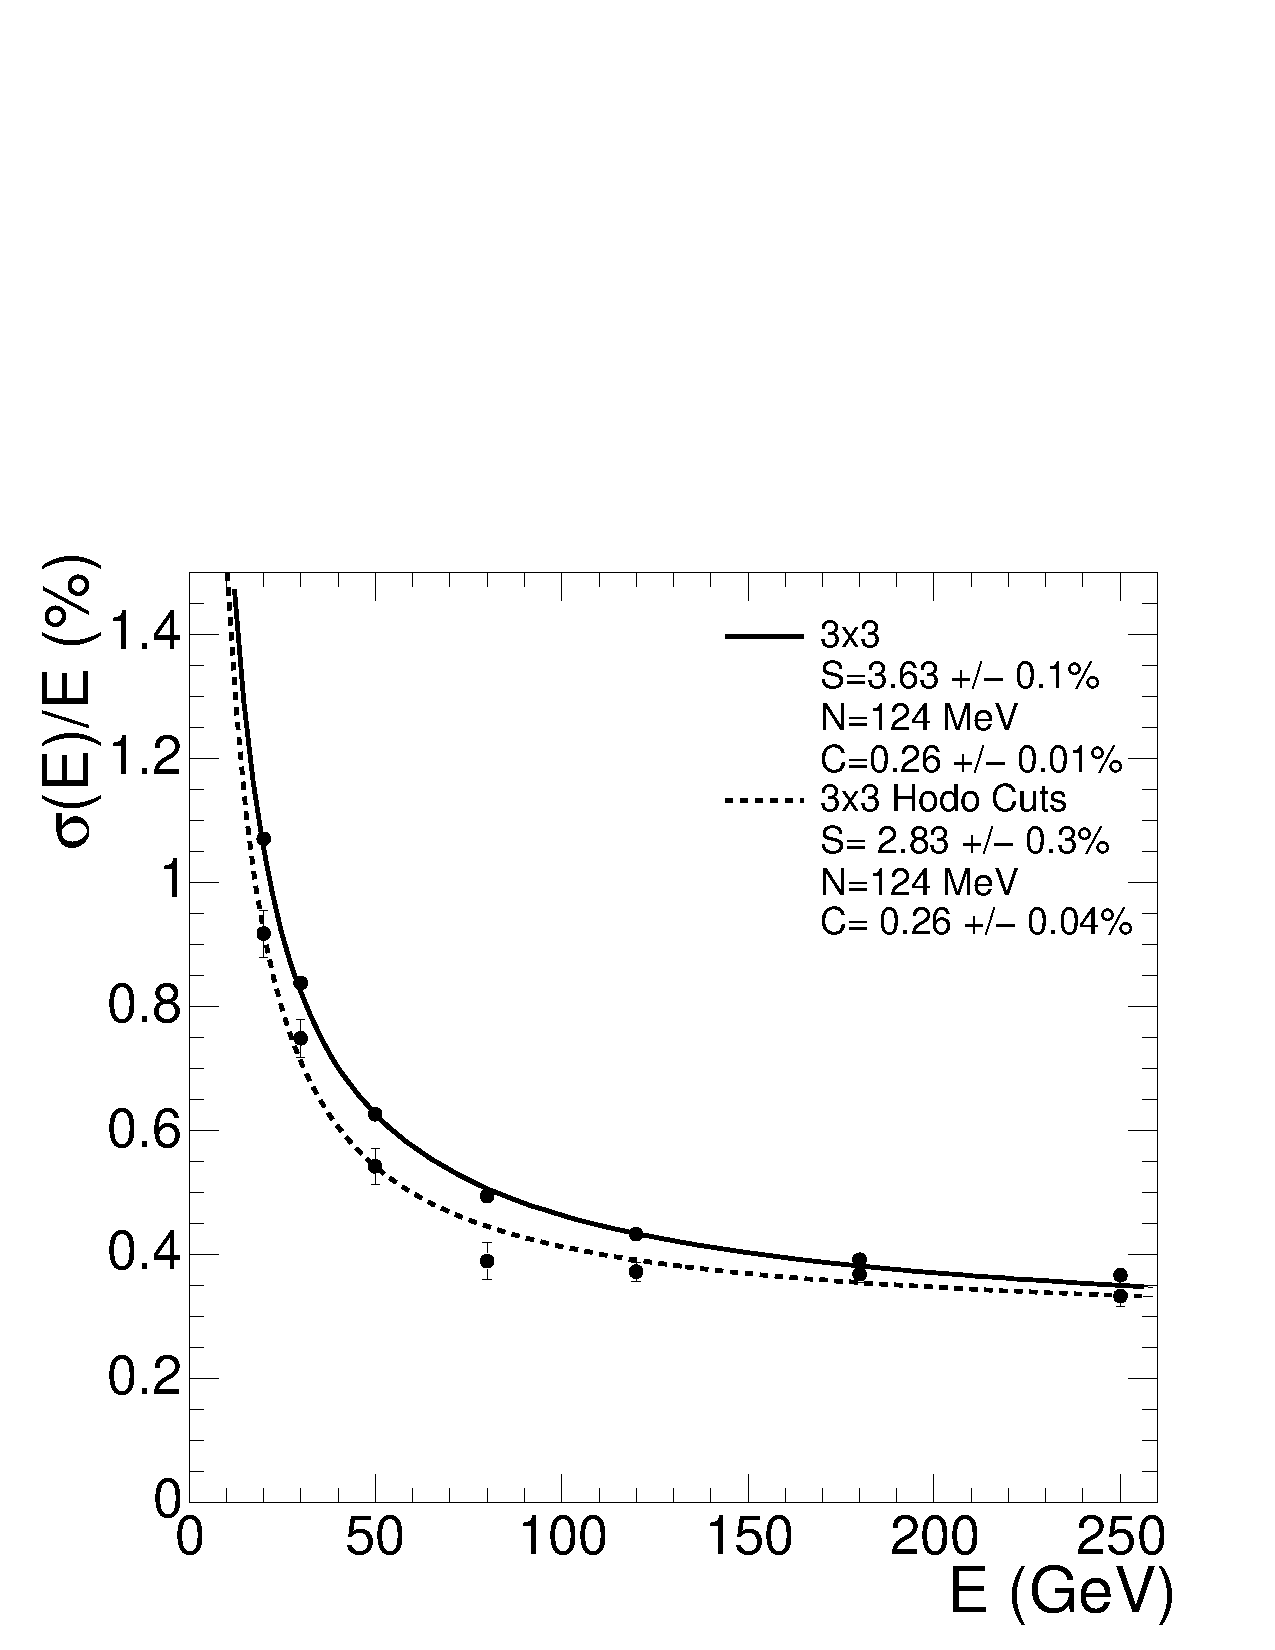
\includegraphics[width=0.7\textwidth]{ecal_performance}
  \caption[Energy resolution $\nicefrac{\sigma}{E}$ of ECAL as a function of
electron energy $E$]{Energy resolution $\nicefrac{\sigma}{E}$ of ECAL as a
function of \label{fig:ECAL} electron energy $E$. From
\cite{chatrchyan2008cms}.}
\end{figure}

\subsection{Hadronic Calorimeter}
The hadronic calorimeter (HCAL), in addition to the electromagnetic calorimeter,
is designed to measure the energy of hadron jets and the missing transverse
energy (\met) which are important signatures in many physics studies at the LHC.

The {HCAL} is a brass/scintillator
sampling hadron calorimeter that covers the region up to $|\eta|<3.0$.  The
scintillation light is channelled by wavelength shifting fibres, that are
embedded in the scintillation tiles, to hybrid photodiodes that can operate in
the high axial magnetic field \cite{chatrchyan2008cms}.

The barrel hadron calorimeter (HB) covers the region ($|\eta| < 1.4$)
and the hadron endcap covers the region $1.4 < |\eta| < 3.0$.

The barrel hadron calorimeter is positioned between the ECAL and the inside of
the solenoid magnet coil ($\unit{1.77}{\meter}<r<\unit{2.95}{\meter}$).  The
strong constraints imposed by the dimensions of the solenoid magnet results in
the HB having an insufficient amount of material to absorb the hadronic shower
in the central region.  To overcome this limitation the outer hadronic
calorimeter (HO) or tail catcher, has been added around the solenoid magnet to
increase the effective thickness of the hadron calorimetry to over 10
interaction lengths.  This provides better protection against punch-through to
the muon system.

\subsubsection{The Forward Calorimeter}
In the forward region ($|\eta| > 3$) energy measurements are made with the
forward hadronic calorimeter, situated \unit{11}{\meter} from the interaction
point. The main role of the forward calorimeter is to improve the \ETm
measurement and to tag jets in the forward direction.

The forward hadronic calorimeter is an iron/quartz-fibre calorimeter where the
Cherenkov light is detected by photomultipliers.  The calorimeter needs to be
radiation hard due to the very large flux in the forward region. However, it is
still expected that after 10 years of operation the light output will be reduced by
about $30\%$ due to the level of radiation \cite{chatrchyan2008cms}. 

\subsubsection{Performance}

\FigureRef{fig:hcalperform} shows the jet energy resolution for three parts of
the {HCAL} measured in test beams. The granularity of the sampling in each
region of the HCAL is such that the resolution is similar in each.

\begin{figure}[htbp]
  \centering
  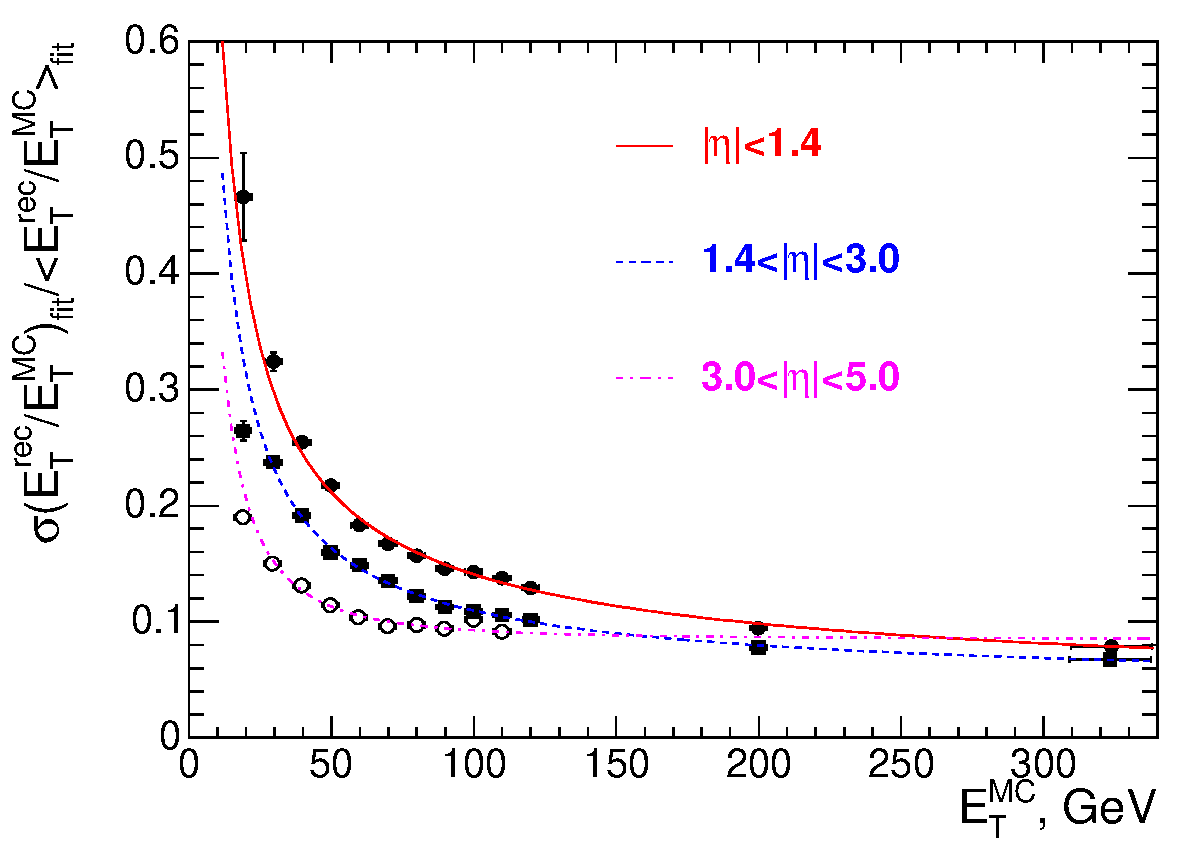
\includegraphics[width=0.7\textwidth]{hcal_performance}
  \caption[The jet transverse energy resolution as a function of jet transverse
energy.] {The jet transverse energy resolution as a function of jet transverse
energy for barrel jets ($|\eta| < 1.4$), endcap jets ($1.4<|\eta| < 3$) and
forward jets ($3<|\eta| < 5$). From \cite{chatrchyan2008cms}. }
  \label{fig:hcalperform}
\end{figure}

\begin{figure}[htbp]
  \centering
  \begin{subfigure}{0.48\textwidth}
    \centering
    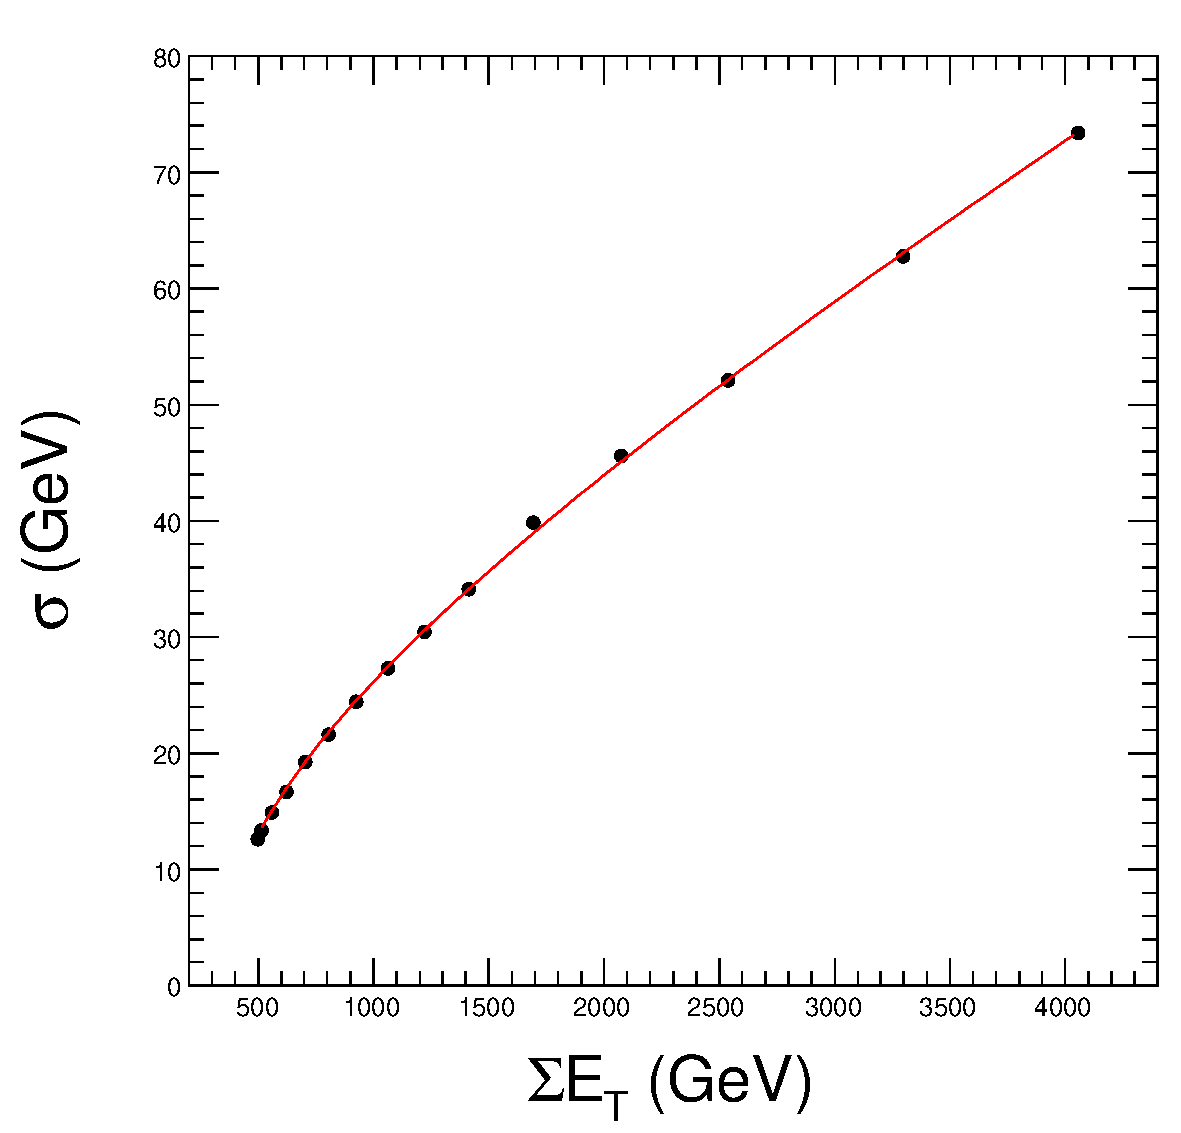
\includegraphics[width=\textwidth]{met_res}
    \caption{\ETm resolution.}
    \label{fig:met_res}
  \end{subfigure}
  \begin{subfigure}{0.48\textwidth}
    \centering
    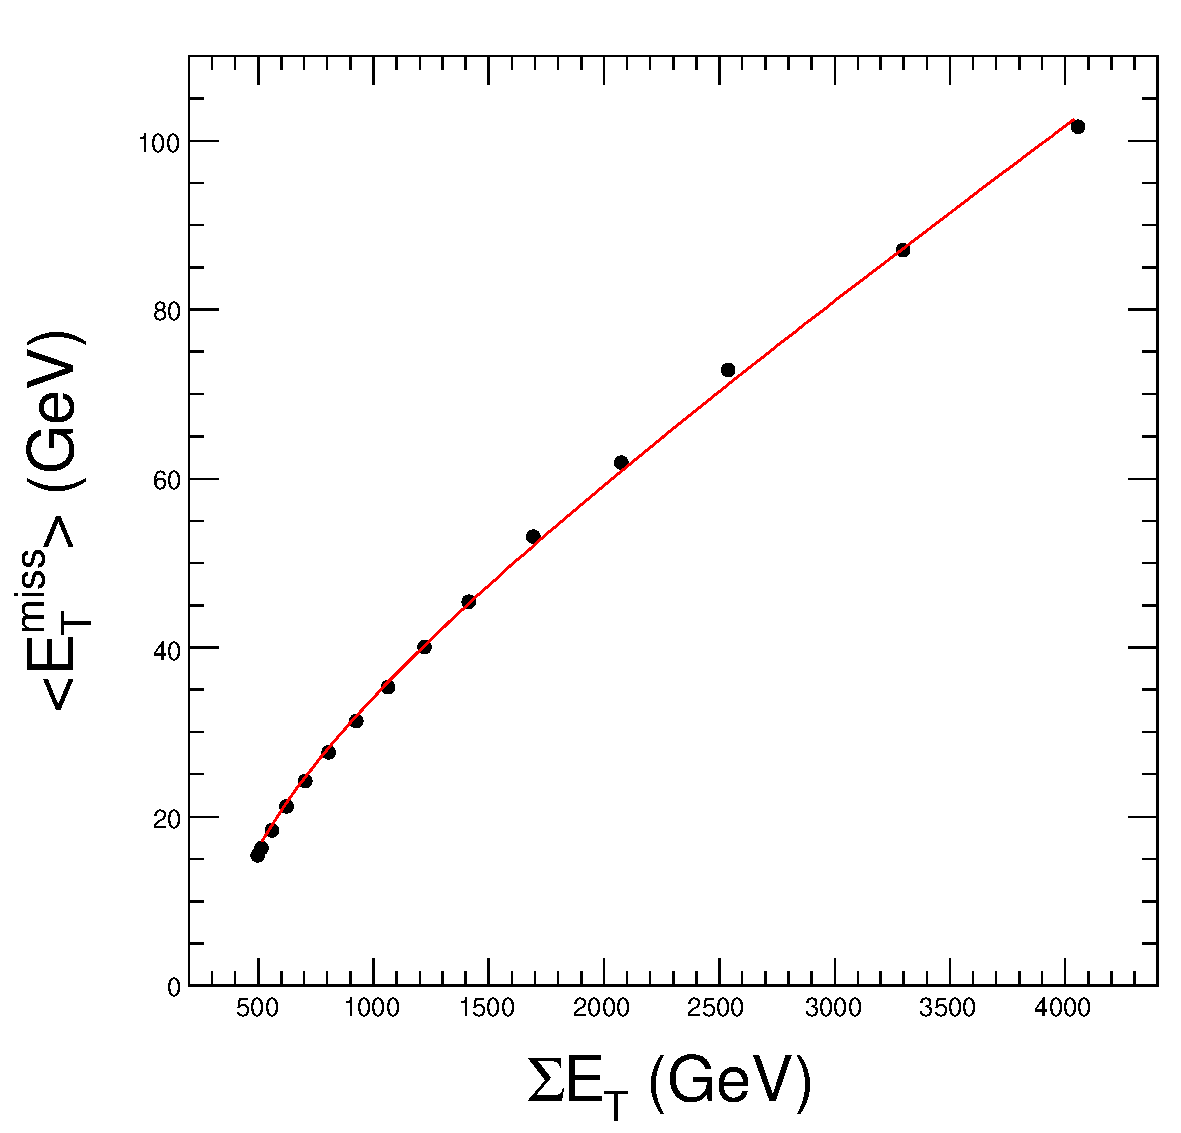
\includegraphics[width=\textwidth]{met_mean}
    \caption{Average reconstructed \ETm.}
    \label{fig:met_mean}
  \end{subfigure}
  \caption[The missing transverse energy performance as a function of the $\sum
E_T$ for QCD events.] { The missing transverse energy performance as a function
of the $\sum E_T$ for QCD events with pile-up. From \cite{chatrchyan2008cms}. }
  \label{fig:met_performance} 
\end{figure}

The performance of the missing transverse energy (\ETm) is shown in
\FigureRef{fig:met_performance} in QCD events. The \ETm resolution is
$\sigma(\ETm) \approx 1.0 \sqrt \ET$ and the average \ETm is 
$\langle \ETm \rangle \approx 1.25 \sqrt \ET$ \cite{chatrchyan2008cms}.
\todo{UNDERSTAND THIS, should etmiss be 0?}

\subsection{Muon System}
The muon system lies outside of the CMS solenoid and the outer HCAL detectors.
It is designed to have three functions; to identify muons, measure the momentum
of muons and trigger on muons. To perform these functions the muon system
consists of several different types of detectors due to the different background
rates and magnetic fields in each region of the detector.
The layout of the {CMS} muon system is shown in \FigureRef{fig:muon_system}.

\begin{figure}[htbp]
  \centering
  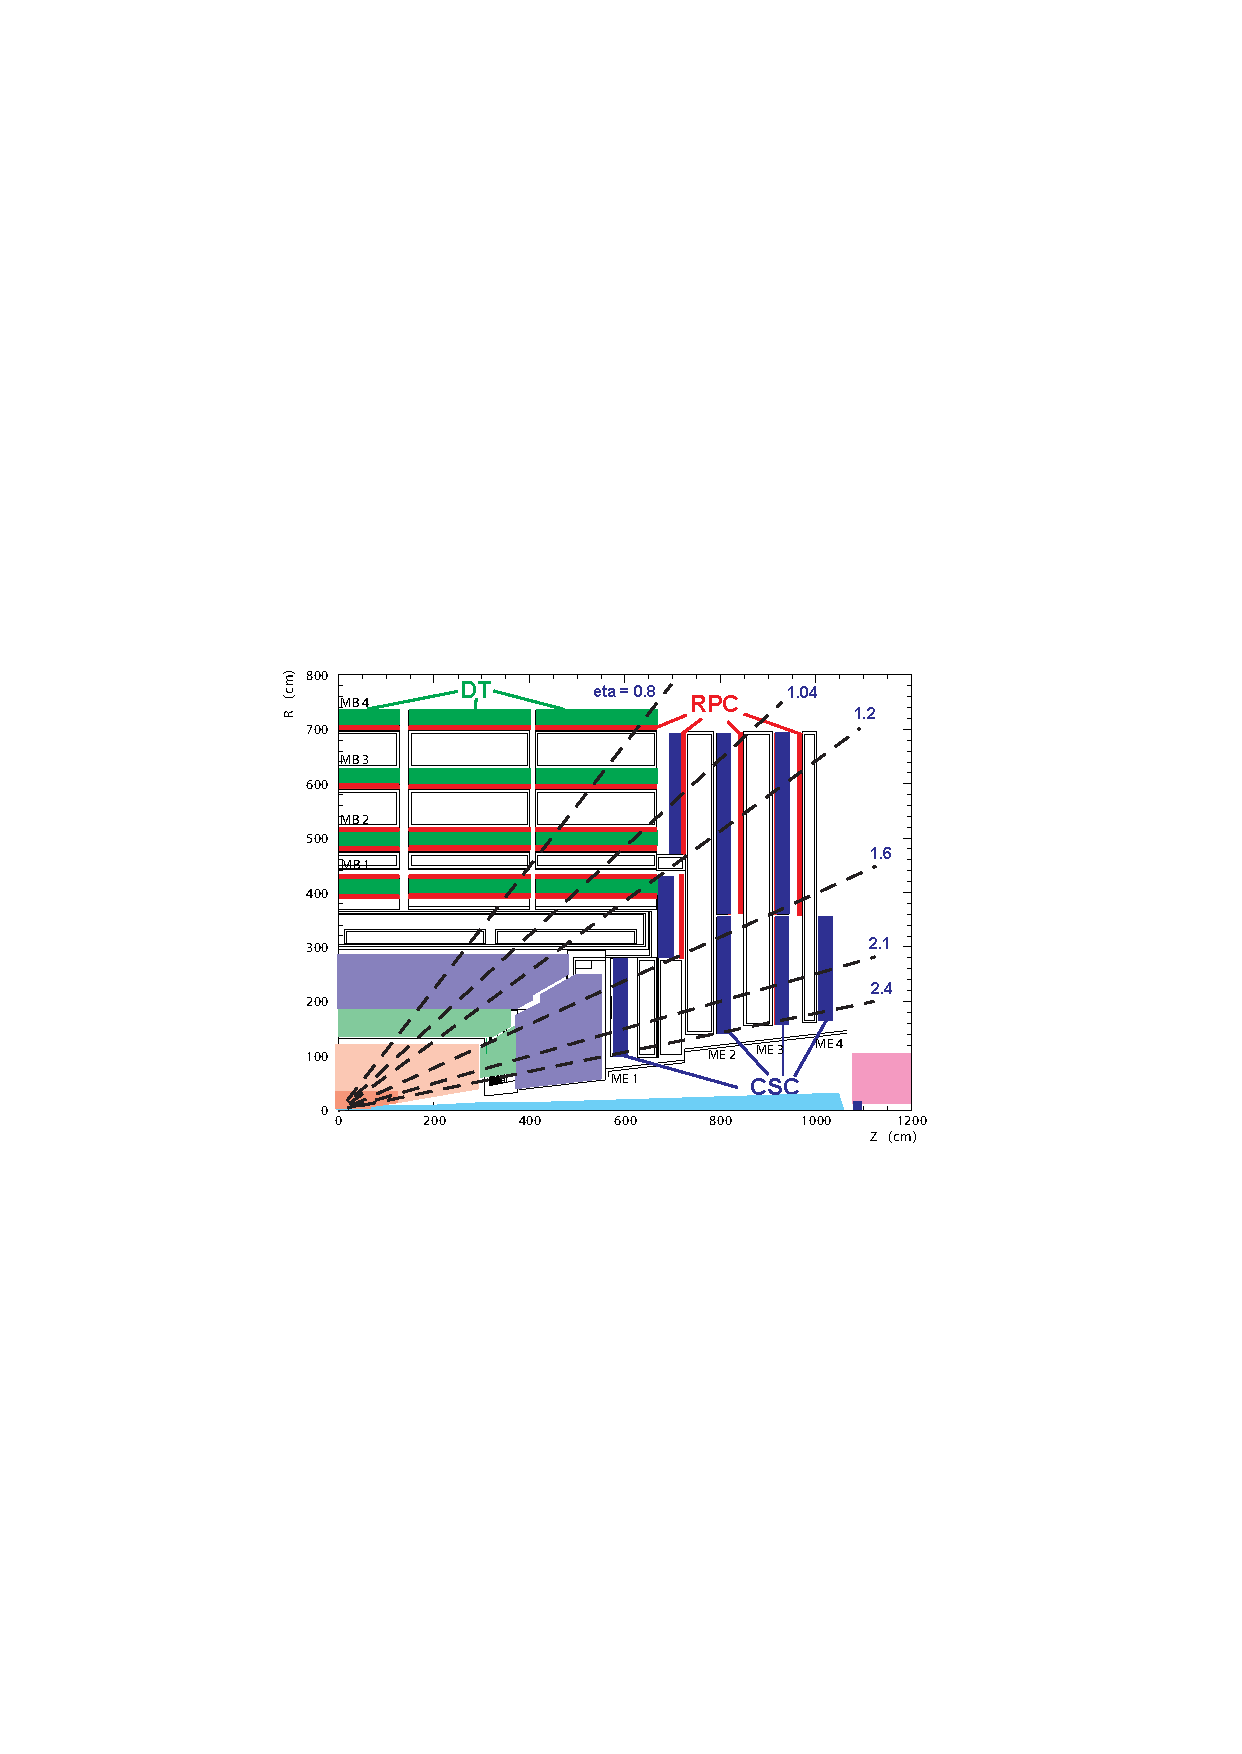
\includegraphics[width=0.98\textwidth]{muon_system}
  \caption[The layout of a quarter of the CMS muon system.] {The layout of a
quarter of the CMS muon system. From \cite{chatrchyan2008cms}.}
  \label{fig:muon_system}
\end{figure}

\subsubsection{Drift Tubes}
In the barrel region ($|\eta| < 1.2$)
where the background rate is low and the residual magnetic field is small,
 aluminium drift tubes (DT) are used,
arranged in four stations interleaved in the flux return
plates. 
Each station contains 12 layers, eight to measure the coordinate in the
$r-\phi$ plane and four to measure the $z$ direction (except the fourth station
which only measures the $r-\phi$ plane). 

\subsubsection{Cathode Strip Chambers}
In the endcaps ($0.9<|\eta|<2.4$), where the muon and background rate is high and
the magnetic field is also high,
cathode strip chambers (CSC) are used. The
CSCs are arranged in four stations in each endcap. Their faces are perpendicular
to the beam line, and are placed between the flux return plates.  The cathode
strips of each chamber run radially away from the beam line whereas the anode
wires run perpendicular to the strips; both are read out which gives information
on both the $r-\phi$ plane (from the cathode) and the $\eta$ direction (from the
anode). \cite{chatrchyan2008cms}

\subsubsection{Resistive Plate Chambers}
In addition to DT chambers and CSCs a complementary trigger system is also used
consisting of resistive plate chambers (RPC) in the endcap and barrel regions.
The RPCs are able to provide a fast and independent trigger over a large range
($|\eta| < 1.6$). In the barrel region, 6 layers of RPCs are used, 2 in each of
the first 2 muon stations and 1 in each of the last 2 stations. In the endcap
there is a layer of RPCs in each of the first 3 stations.

\subsubsection{Alignment}
An optical alignment system, that uses lasers and LEDs, measures the position
of each muon station with respect to each other and the CMS inner tracker to
ensure an accurate and high resolution measurement of the muon
momentum.\cite{chatrchyan2008cms}

\subsubsection{Performance}
The performance of the muon system and inner tracker is shown in 
\FigureRef{fig:muon_performance}. The best momentum resolution for low-momentum muons
is obtained from the measurement in the silicon tracker. However, as the momentum
increases the muon momentum resolution is best measured by combining information
from both the inner tracker and the muon detector.

\begin{figure}[htbp]
  \centering
  \begin{subfigure}{0.48\textwidth}
    \centering
    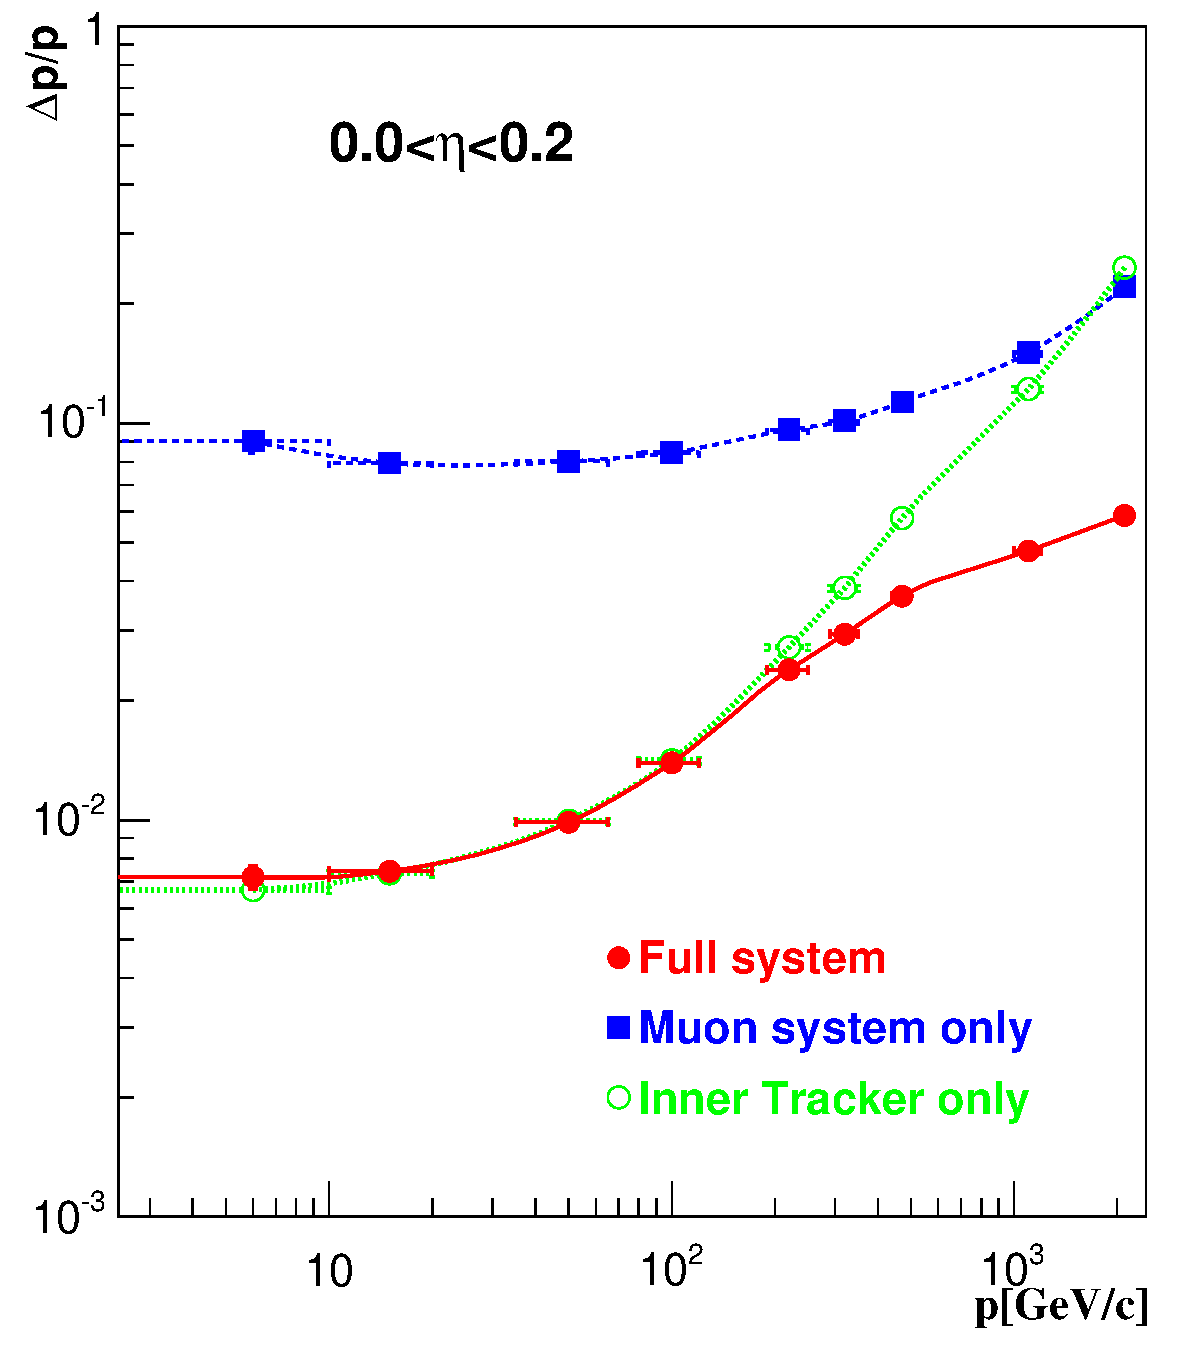
\includegraphics[width=\textwidth]{muon_barrel}
    \caption{Barrel.}
    \label{fig:muon_barrel}
  \end{subfigure}
  \begin{subfigure}{0.48\textwidth}
    \centering
    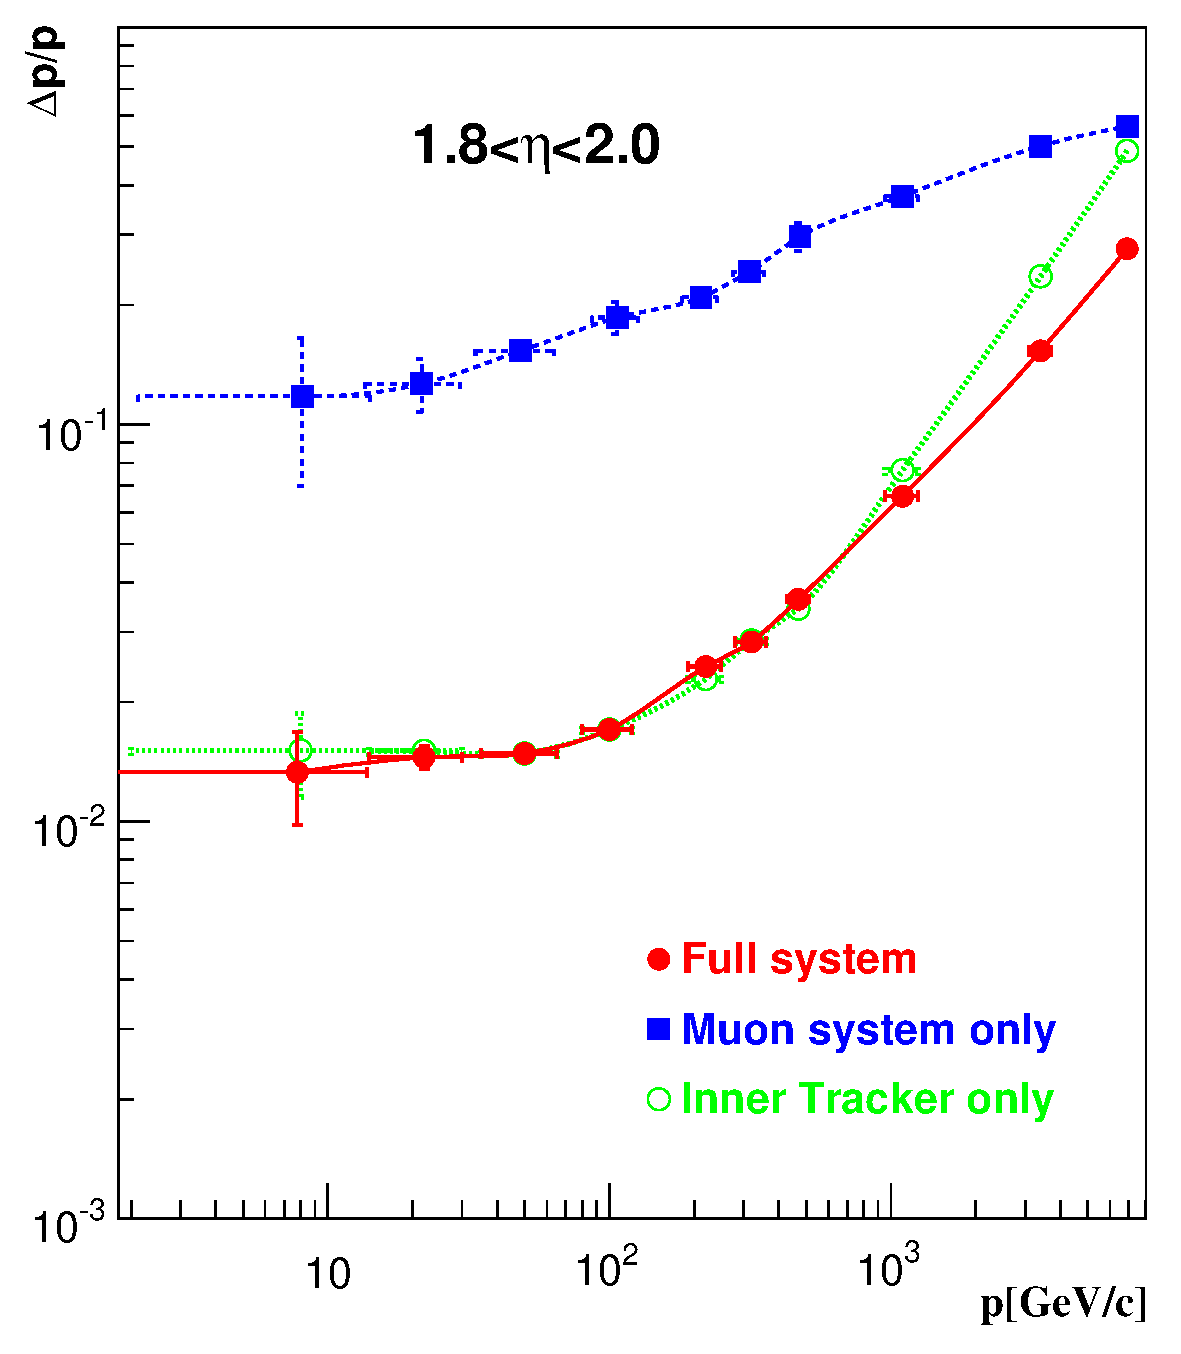
\includegraphics[width=\textwidth]{muon_endcap}
    \caption{Endcap.}
    \label{fig:muon_endcap}
  \end{subfigure}
  \caption[Muon transverse momentum resolution as a function of the muon
momentum.] {Muon transverse momentum resolution as a function of the muon
momentum using only the muon system, only the tracker and both, for barrel muons
($|\eta| < 0.8$) and endcap muons ($1.2<|\eta| < 2.4$). From
\cite{chatrchyan2008cms}.\label{fig:muon_performance}}
\end{figure}

\subsection{Trigger and Data Acquisition}
At design luminosity, the high bunch crossing frequency of the LHC means that
each crossing will contain an average of 20 superimposed inelastic
events every \unit{25}{\nano\second}, a rate of $10^{9}$ interactions per
second.
The size of an event is approximately \unit{1}{\mega\bel} after zero-suppression.
The total data output rate from CMS is \unit{$\approx 80$}{\tera\bel\per\second}.
These figures are many orders of magnitude larger that the storage and offline
processing capability available to CMS, which corresponds to about
\unit{250}{\mega\bel\per\second} or about $\approx 10^{2}$ crossings written to the tape
storage every second. 

The vast majority of events will contain only glancing inelastic collisions and
may not be of interest from a physics perspective and can be discarded.  It is
the job of the trigger to reduce the rate of events by a factor of $10^6$ by
rejecting the uninteresting events while keeping as many interesting events as
possible.

An overview of the {DAQ} and trigger is shown in figure \ref{fig:CMSDAQ}.
The trigger is separated into two parts; the Level-1 (L1) trigger and the High
Level Trigger (HLT).\cite{chatrchyan2008cms}

\begin{figure}[htbp]
  \centering
  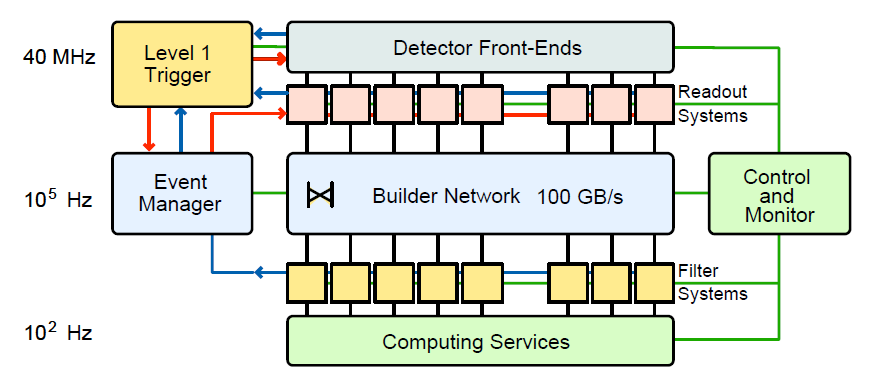
\includegraphics[width=0.98\textwidth]{CMSDAQ}
  \caption[Overview of the architecture of the CMS DAQ and trigger.] {Overview
of the architecture of the CMS DAQ and trigger. From \label{fig:CMSDAQ}
\cite{chatrchyan2008cms}.}
\end{figure}

\subsubsection{Level-1 Trigger}

The Level-1 trigger (L1) is designed to reduce the event rate from the bunch
crossing frequency of \unit{40}{\mega\hertz} to a maximum output rate of
\unit{100}{\kilo\hertz}.  The L1 trigger is implemented with custom-designed
fast programmable electronics that takes as input coarse data from the
calorimeters and muon systems; the high resolution data are placed in pipe-lined
memories awaiting a Level-1 decision. The reduced resolution and granularity data are used to form ``trigger
primitives'', such as isolated high energy electromagnetic deposits that pass a
certain \PT or \ET threshold, which the L1 Trigger uses to base its decision. It
also receives information on event-wide variables such as the total sum of
transverse energy and the missing transverse energy.
\todo{trigger tables?}

\subsubsection{High-Level Triggers}
After a fixed time interval of \unit{3.2}{\micro\second} the high resolution
event data held in the pipeline memories is either read out or discarded
depending on the decision at the Level-1 trigger.  The data are transferred to a
processor running the high-level trigger software.

The high-level trigger (HLT) is a software system which runs on a server farm
with over one thousand commercial multicore processors with access to the
complete event data allowing it to make more complex calculations. 
Objects are reconstructed in the HLT as they are needed and events are discarded
as soon as possible to avoid wasting processing time.
The decision to accept an event is based on the requirements on the datasets
used in {CMS} analyses. A typical data-set requires a high \pT
HLT-reconstructed object or an amount of missing transverse energy in the event.
For example, the data-set relevant to the analyses that follow in later chapters
requires a single high \pT electron.
\todo{good to add a table or point to selection of W}

\subsubsection{Computing}

The {CMS} data is available in several different file formats that contain
different levels of details \cite{grandi2004cms},
\begin{itemize}
\item Raw data, is the output of the events that pass the {HLT}. The files
contain the detector data, the {L1} trigger results, the {HLT} trigger
results and the higher-level objects that are created during the {HLT}
process.
\item Reconstructed (RECO) data, is the output of the reconstruction process.
The files contain the reconstructed physics objects and reconstructed hits and
clusters.
\item Analysis Object Data (AOD), is the reduced event representation and
contains only the reconstructed objects. This is the format that is used to
perform physics analyses.
\end{itemize}

CMS utilises a distributed computing model called the ``Grid''.  The Grid
consists of several clusters of computers distributed around the world and
organised into several tiers \cite{grandi2004cms}.  Events that pass the {HLT}
are sent to the primary Tier-0 centre where the raw data are stored on tape
before undergoing prompt reconstruction. The reconstructed data are distributed
to Tier-1 and Tier-2 centres at national laboratories and universities around the
world. The role of the Tier-1 and Tier-2 sites are to run the physics analyses
and to reprocess the data when updated calibrations are available. This is
typically done once or twice a year.

